% ============================================================
%  Estadística · LCC · Universidad de Sonora
%  Semana 2 — Unidad 1 completa y comienzo de la Unidad 2
%  Archivo autocontenido. Se puede copiar y pegar tal cual en Overleaf.
% ============================================================
\documentclass[aspectratio=169,10pt]{beamer}
\usepackage[utf8]{inputenc}
\usepackage[T1]{fontenc}
\usepackage[spanish,es-nodecimaldot,es-noquoting]{babel}
\usepackage{lmodern}
\usepackage{amsmath,amssymb}
\usepackage{booktabs}
\usepackage{tikz}
\usepackage{listings}
\usepackage{graphicx}
\graphicspath{{figuras/}}
% ------------------------------------------------------------
%  ILUSTRACIONES DE palmerpenguins
%  Ejecutar una vez  presentaciones/copiar-figuras.R  para obtenerlas.
%  Si no están presentes, las diapositivas compilan igual usando los
%  dibujos en TikZ definidos más abajo.
%  Crédito obligatorio: Artwork by @allison_horst
% ------------------------------------------------------------
\newcommand{\creditoHorst}{{\tiny\color{grisT} Ilustración: \textit{Artwork by @allison\_horst}}}
% ---------- Tema y colores ----------
\usetheme{default}
\setbeamertemplate{navigation symbols}{}
\definecolor{azulUS}{HTML}{1F4E79}
\definecolor{azulClaro}{HTML}{DCE6F1}
\definecolor{grisT}{HTML}{5F5E5A}
\definecolor{negroP}{HTML}{2B2B2B}
\definecolor{picoNaranja}{HTML}{E8871E}
\definecolor{rosaK}{HTML}{F4A6B8}
\definecolor{verdeOk}{HTML}{1D9E75}
\definecolor{rojoAc}{HTML}{C0392B}
\definecolor{grisR}{HTML}{9A9A9A}
\definecolor{azulR}{HTML}{2266B3}
\setbeamercolor{structure}{fg=azulUS}
\setbeamercolor{frametitle}{fg=white,bg=azulUS}
\setbeamercolor{title}{fg=azulUS}
\setbeamerfont{frametitle}{size=\large,series=\bfseries}
\setbeamertemplate{frametitle}{%
  \nointerlineskip
  \begin{beamercolorbox}[wd=\paperwidth,ht=2.6ex,dp=1.2ex,leftskip=0.3cm]{frametitle}
    \usebeamerfont{frametitle}\insertframetitle
  \end{beamercolorbox}}
\setbeamertemplate{footline}{%
  \hfill\textcolor{grisT}{\tiny Estadística · LCC · Unison \quad
  \insertframenumber/\inserttotalframenumber}\hspace{0.3cm}\vspace{0.15cm}}
\setbeamertemplate{itemize item}{\textcolor{azulUS}{\raisebox{0.15ex}{\tiny$\blacksquare$}}}
\setbeamertemplate{itemize subitem}{\textcolor{grisT}{\raisebox{0.15ex}{\tiny$\bullet$}}}
% ---------- Estilo para código de R ----------
\lstdefinestyle{Rstyle}{
  language=R, basicstyle=\ttfamily\footnotesize,
  keywordstyle=\color{azulUS}\bfseries, commentstyle=\color{grisT}\itshape,
  stringstyle=\color{verdeOk}, showstringspaces=false, breaklines=true,
  frame=single, rulecolor=\color{azulClaro}, backgroundcolor=\color{azulClaro!35},
  numbers=none, aboveskip=6pt, belowskip=4pt,
  % Para que las vocales acentuadas no rompan la compilación si algún día se
  % escriben dentro de un bloque de código o de un comentario.
  extendedchars=true,
  literate={á}{{\'a}}1 {é}{{\'e}}1 {í}{{\'i}}1 {ó}{{\'o}}1 {ú}{{\'u}}1
           {Á}{{\'A}}1 {É}{{\'E}}1 {Í}{{\'I}}1 {Ó}{{\'O}}1 {Ú}{{\'U}}1
           {ñ}{{\~n}}1 {Ñ}{{\~N}}1 {ü}{{\"u}}1 {Ü}{{\"U}}1
           {¿}{{?`}}1 {¡}{{!`}}1}
\lstset{style=Rstyle}
% ---------- Comandos de R dentro del texto ----------
%  Mismo aspecto que el código en línea del libro: fondo gris y letra morada.
%  Los valores vienen del tema del libro (--bs-code-color: #7D12BA). El gris se
%  oscureció un poco respecto al de la web (#F8F9FA) para que se vea proyectado.
\definecolor{codigoTexto}{HTML}{7D12BA}
\definecolor{codigoFondo}{HTML}{EFF0F2}
\newcommand{\Rc}[1]{{\setlength{\fboxsep}{1.6pt}%
  \colorbox{codigoFondo}{\textcolor{codigoTexto}{\texttt{#1}}}}}
% ---------- Caja auxiliar para destacar ideas ----------
\newcommand{\destaca}[1]{%
  \par\vspace{3pt}\noindent
  \colorbox{azulClaro}{%
    \parbox{\dimexpr\linewidth-2\fboxsep\relax}{\vspace{3pt}#1\vspace{3pt}}}%
  \par\vspace{3pt}}
% ---------- Hojas de separación por sesión ----------
%  Cumplen dos funciones: al preparar la clase, ver de un golpe dónde terminó
%  cada día; al repasar, reconocer dónde empieza cada bloque.
%
%  SIN NUMERAR A PROPÓSITO. El número global de sesión se rompe en cuanto el
%  calendario real se mueve, y se mueve siempre. La hoja marca el corte por su
%  posición, que no depende de ninguna cuenta.
%
%  Uso:  \hojaSesion{Título del bloque}{Resumen de lo que se vio.}
%  Va dentro de un frame [plain]:
%      \begin{frame}[plain]
%        \hojaSesion{...}{...}
%      \end{frame}
\newcommand{\hojaSesion}[2]{%
  \vfill
  \begin{beamercolorbox}[wd=\textwidth,sep=16pt,center]{frametitle}
    {\Large\bfseries #1}\\[11pt]
    \begin{minipage}{0.82\textwidth}\centering\small #2\end{minipage}
  \end{beamercolorbox}
  \vfill}
% ============================================================
%  PINGÜINOS EN TIKZ  (estilo kawaii)
%  Solo se usan como respaldo: si están las ilustraciones de Horst en
%  figuras/, esas tienen prioridad y estos dibujos no aparecen.
% ============================================================
% Cuerpo común. Argumento: color de pico y patas.
\newcommand{\cuerpoPing}[1]{%
  \fill[negroP] (-0.88,0.18) ellipse (0.17 and 0.5);      % ala izquierda
  \fill[negroP] (0.88,0.18) ellipse (0.17 and 0.5);       % ala derecha
  \fill[#1] (-0.28,-1.12) ellipse (0.19 and 0.085);       % pata izquierda
  \fill[#1] (0.28,-1.12) ellipse (0.19 and 0.085);        % pata derecha
  \fill[negroP] (0,0) ellipse (0.82 and 1.1);             % cuerpo
  \fill[white] (0,-0.16) ellipse (0.53 and 0.82);         % vientre
}
% Ojos grandes con brillo y rubor
\newcommand{\ojosPing}{%
  \fill[white] (-0.22,1.3) circle (0.155);
  \fill[white] (0.22,1.3) circle (0.155);
  \fill[negroP] (-0.20,1.28) circle (0.085);
  \fill[negroP] (0.24,1.28) circle (0.085);
  \fill[white] (-0.235,1.315) circle (0.032);
  \fill[white] (0.205,1.315) circle (0.032);
  \fill[rosaK,opacity=0.55] (-0.44,1.10) circle (0.085);
  \fill[rosaK,opacity=0.55] (0.44,1.10) circle (0.085);
}
\newcommand{\picoPing}[1]{%
  \fill[#1] (-0.10,1.13) -- (0.10,1.13) -- (0,0.94) -- cycle;
}
% --- Adelaida (Adelie): cabeza negra, anillo blanco alrededor del ojo
\newcommand{\pingAdelie}{%
  \begin{scope}
    \cuerpoPing{picoNaranja}
    \fill[negroP] (0,1.22) circle (0.6);
    \fill[white] (-0.22,1.3) circle (0.20);
    \fill[white] (0.22,1.3) circle (0.20);
    \ojosPing
    \picoPing{picoNaranja}
  \end{scope}}
% --- Barbijo (Chinstrap): cara blanca con una franja negra bajo el mentón
\newcommand{\pingChinstrap}{%
  \begin{scope}
    \cuerpoPing{picoNaranja}
    \fill[negroP] (0,1.22) circle (0.6);
    \fill[white] (0,1.26) ellipse (0.5 and 0.5);
    \draw[negroP,line width=1.6pt] (-0.44,1.02) arc (205:335:0.48);
    \ojosPing
    \picoPing{negroP}
  \end{scope}}
% --- Juanito (Gentoo): parche blanco sobre los ojos y pico naranja
\newcommand{\pingGentoo}{%
  \begin{scope}
    \cuerpoPing{picoNaranja}
    \fill[negroP] (0,1.22) circle (0.6);
    \fill[white] (-0.26,1.5) ellipse (0.21 and 0.13);
    \fill[white] (0.26,1.5) ellipse (0.21 and 0.13);
    \fill[white] (0,1.56) ellipse (0.3 and 0.075);
    \ojosPing
    \picoPing{picoNaranja}
  \end{scope}}
% ============================================================
%  ICONOS DE R Y RSTUDIO
%  Aproximaciones estilizadas hechas en TikZ. Si se prefieren los
%  logotipos oficiales, están disponibles en r-project.org (CC-BY-SA)
%  y en posit.co; bastaría guardarlos en figuras/ e incluirlos.
% ============================================================
\newcommand{\iconoR}{%
  \begin{scope}
    \fill[grisR] (0,0) ellipse (0.72 and 0.50);
    \fill[white] (0,0) ellipse (0.50 and 0.31);
    \node[azulR,font=\bfseries\large] at (0.02,0.02) {R};
  \end{scope}}
\newcommand{\iconoRStudio}{%
  \begin{scope}
    \fill[azulR] (0,0) circle (0.52);
    \fill[white] (0,0) circle (0.40);
    \node[azulR,font=\bfseries] at (0,0.02) {R};
    \draw[azulR,line width=1.3pt] (-0.20,-0.26) -- (0.28,-0.26);
  \end{scope}}
% ============================================================
\title{\LARGE\textbf{Estadística}}
\subtitle{Licenciatura en Ciencias de la Computación}
\author{Prof. Rosalía Gpe. Hernández Amador}
\institute{Departamento de Matemáticas · Universidad de Sonora}
\date{Semestre 2026-2}
\begin{document}
% ============================================================
\section{Unidad 1: Exploración de los datos}
\begin{frame}[plain]
  \centering

  \vspace{1.2cm}
  {\Large\bfseries\color{azulUS} Unidad 1}\\[6pt]
  {\large\color{azulUS} Exploración de los datos}\\[14pt]
  \IfFileExists{figuras/lter_penguins.png}{%
    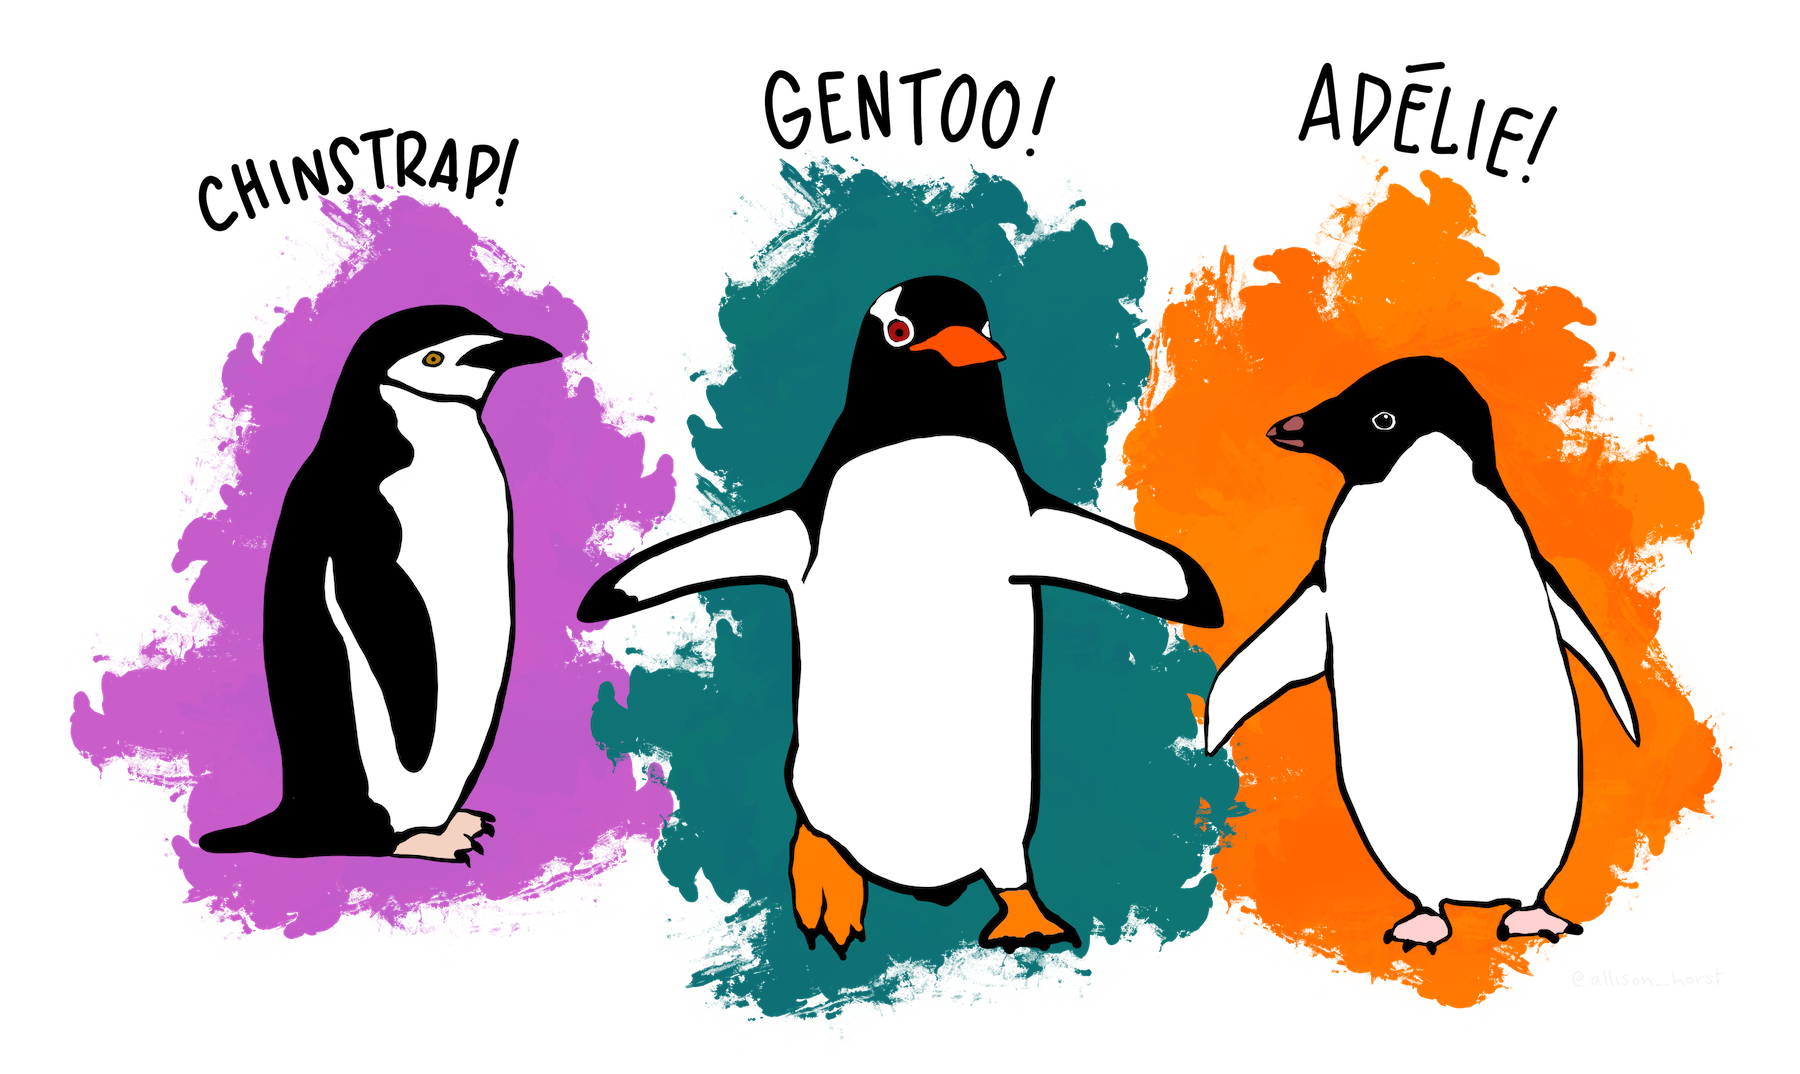
\includegraphics[height=0.32\textheight]{lter_penguins.png}
  }{%
    \begin{tikzpicture}[scale=0.55]
      \begin{scope}[shift={(-2,0)}] \pingAdelie \end{scope}
      \begin{scope}[shift={(0,0)}] \pingChinstrap \end{scope}
      \begin{scope}[shift={(2,0)}] \pingGentoo \end{scope}
    \end{tikzpicture}
  }\\[10pt]
  {\small\color{grisT} Aprender a mirar los datos antes de tocarlos}
\end{frame}
\begin{frame}{Todo empieza con una tabla}
  \centering
  {\footnotesize
  \begin{tabular}{@{}lllccc@{}}
    \toprule
    \textbf{especie} & \textbf{isla} & \textbf{sexo} & \textbf{pico (mm)} & \textbf{aleta (mm)} & \textbf{masa (g)} \\
    \midrule
    Adelia & Torgersen & macho & 39.1 & 181 & 3750 \\
    Adelia & Torgersen & hembra & 39.5 & 186 & 3800 \\
    Juanito & Biscoe & hembra & 46.1 & 211 & 4500 \\
    Barbijo & Dream & macho & 50.0 & 196 & 3900 \\
    \multicolumn{6}{c}{\textcolor{grisT}{\textit{... 340 renglones más}}} \\
    \bottomrule
  \end{tabular}}

  \vspace{0.7cm}
  \raggedright
  \begin{columns}[T]
    \begin{column}{0.48\textwidth}
      \destaca{\textbf{Individuos} (los renglones)\\[3pt]
      {\small Cada renglón es \emph{un pingüino}: la unidad que observamos}}
    \end{column}
    \begin{column}{0.48\textwidth}
      \destaca{\textbf{Variables} (las columnas)\\[3pt]
      {\small Cada columna es \emph{algo que medimos} de cada pingüino}}
    \end{column}
  \end{columns}
\end{frame}
\begin{frame}{Confundir esto es el error número uno}
  \destaca{\textbf{Pregunta.} En los datos de la cata de galletas, ¿qué es un individuo:
  una marca de galleta o la calificación de un juez?}

  \vspace{0.8cm}
  \pause
  Es \textbf{cada calificación}: un renglón por juez y por marca.

  \vspace{0.4cm}
  \centering
  {\footnotesize
  \begin{tabular}{@{}cccc@{}}
    \toprule
    \textbf{juez} & \textbf{orden} & \textbf{marca} & \textbf{agrado} \\
    \midrule
    1 & 1 & Oreo & 8 \\
    1 & 2 & Chokis & 7 \\
    1 & 3 & Lors & 5 \\
    2 & 1 & Lors & 6 \\
    \bottomrule
  \end{tabular}}

  \vspace{0.5cm}
  \raggedright
  {\footnotesize Si la tabla estuviera armada con un renglón por marca, no podríamos
  analizar nada: perderíamos la información de quién calificó qué.}
\end{frame}
\begin{frame}{Tipos de variables}
  \begin{columns}[T]
    \begin{column}{0.48\textwidth}
      \destaca{\textbf{Categóricas} (cualitativas)\\[4pt]
      {\small Clasifican al individuo en grupos\\[4pt]
      \textit{especie, isla, sexo, marca de galleta}}}
    \end{column}
    \begin{column}{0.48\textwidth}
      \destaca{\textbf{Cuantitativas} (numéricas)\\[4pt]
      {\small Miden una cantidad\\[4pt]
      \textit{masa, largo de la aleta, tiempo de ejecución}}}
    \end{column}
  \end{columns}

  \vspace{0.7cm}
  \destaca{\textbf{Cuidado.} No todo número es cuantitativo. El \emph{año} de observación
  es un número, pero promediar años rara vez tiene sentido. Y un código de muestra
  como \texttt{G134} es una etiqueta, no una cantidad.}
\end{frame}
\begin{frame}{Escalas de medición}
  \centering
  {\small
  \begin{tabular}{@{}llp{5.2cm}@{}}
    \toprule
    \textbf{Escala} & \textbf{Permite} & \textbf{Ejemplo} \\
    \midrule
    \textbf{Nominal}   & Solo distinguir categorías & Especie, isla, marca \\
    \textbf{Ordinal}   & Ordenar, sin distancias definidas & Nivel de agrado: bajo, medio, alto \\
    \textbf{Intervalo} & Orden y distancias, sin cero absoluto & Temperatura en $^\circ$C \\
    \textbf{Razón}     & Orden, distancias y cero absoluto & Masa, longitud, tiempo \\
    \bottomrule
  \end{tabular}}

  \vspace{0.6cm}
  \raggedright
  \destaca{La escala decide qué operaciones tienen sentido. Promediar temperaturas
  corporales es válido; ``promediar'' especies, no.

  \vspace{0.2cm}
  ¿Y la escala hedónica de la cata, de 1 a 7? Estrictamente es \textbf{ordinal}, pero
  en análisis sensorial se trata como cuantitativa por convención. Es una decisión
  que conviene hacer explícita, no esconder.}
\end{frame}
\begin{frame}{Ejercicio rápido de clasificación}
  \centering
  {\small
  \begin{tabular}{@{}lcc@{}}
    \toprule
    \textbf{Variable} & \textbf{¿Tipo?} & \textbf{¿Escala?} \\
    \midrule
    Especie del pingüino & & \\[6pt]
    Masa corporal en gramos & & \\[6pt]
    Nivel de dulzor preferido (poco / medio / muy) & & \\[6pt]
    Código de la muestra (\texttt{G134}) & & \\[6pt]
    Número de galletas consumidas al mes & & \\
    \bottomrule
  \end{tabular}}

  \vspace{0.7cm}
  \raggedright
  {\footnotesize Se resuelve en voz alta. La última tiene trampa: es cuantitativa
  \emph{discreta} y de razón.}
\end{frame}
\begin{frame}{¿De dónde vienen los datos? Dos mundos distintos}
  \begin{columns}[T]
    \begin{column}{0.48\textwidth}
      \destaca{\textbf{Estudio observacional}\\[4pt]
      {\small Medimos \textbf{sin intervenir}.\\[4pt]
      \textit{Comparar la temperatura de lagartijas de ciudad y de campo:
      nadie decidió dónde vive cada una.}}}

      \vspace{0.3cm}
      \centering\textcolor{rojoAc}{\small Permite hablar de \textbf{asociación}}
    \end{column}
    \begin{column}{0.48\textwidth}
      \destaca{\textbf{Experimento}\\[4pt]
      {\small \textbf{Aplicamos tratamientos} y medimos la respuesta.\\[4pt]
      \textit{Decidir al azar en qué orden cata cada juez las cuatro marcas.}}}

      \vspace{0.3cm}
      \centering\textcolor{verdeOk}{\small Permite hablar de \textbf{causa y efecto}}
    \end{column}
  \end{columns}

  \vspace{0.6cm}
  \destaca{Un titular como \textit{``quienes toman café viven más''} viene de un estudio
  \textbf{observacional}. Quizá quienes toman café comparten otros hábitos, y esos
  explican la diferencia. Por eso el titular no autoriza a concluir que el café alargue la vida.}
\end{frame}
% ============================================================
%  Este frame estaba antes en la presentación del curso. Se movió aquí, justo
%  después de definir observacional y experimento, para no adelantar los términos
%  tratamiento, azar, causa y efecto en la primera media hora de clase.
% ============================================================
\begin{frame}{Nuestros dos conjuntos, uno de cada tipo}
  \begin{columns}[T]
    \begin{column}{0.48\textwidth}
      \destaca{\textbf{Un estudio bien diseñado}\\[4pt]
      {\small El de los pingüinos. Se planeó todo con cuidado: qué medir, con qué
      instrumento, en qué etapa, cuántos nidos por isla.

      \vspace{0.2cm}
      Pero nadie \emph{asignó} la especie ni el sexo de cada pingüino: eso ya venía dado.}}

      \vspace{0.25cm}
      \centering\textcolor{rojoAc}{\small Sigue siendo \textbf{observacional}}
    \end{column}
    \begin{column}{0.48\textwidth}
      \destaca{\textbf{Un experimento}\\[4pt]
      {\small La cata de galletas. Nosotros decidiremos, \emph{al azar}, en qué orden
      prueba cada juez cada marca.

      \vspace{0.2cm}
      Al asignar nosotros los tratamientos, podremos hablar de causa.}}

      \vspace{0.25cm}
      \centering\textcolor{verdeOk}{\small Es un \textbf{experimento}}
    \end{column}
  \end{columns}

  \vspace{0.45cm}
  \destaca{Conviene no confundir \emph{planear bien la recolección} con \emph{hacer un
  experimento}. El estudio de los pingüinos es un ejemplo excelente de lo primero, y de
  ahí salieron respuestas válidas a sus preguntas. Pero solo la asignación al azar de
  tratamientos (lo que haremos con las galletas) autoriza a hablar de \textbf{causa y efecto}.}
\end{frame}
\begin{frame}{Tres formas de obtener datos}

  \vspace{0.2cm}
  \centering
  \begin{tikzpicture}[scale=0.95]
    \node[fill=azulClaro,rounded corners,text width=3.3cm,align=center,minimum height=1.9cm] at (-4.2,0)
      {\textbf{Censo}\\[3pt]{\scriptsize Se mide \emph{toda} la población}\\[3pt]{\scriptsize Caro, a veces imposible}};
    \node[fill=azulClaro,rounded corners,text width=3.3cm,align=center,minimum height=1.9cm] at (0,0)
      {\textbf{Muestra}\\[3pt]{\scriptsize Se mide una \emph{parte} bien elegida}\\[3pt]{\scriptsize Unidad 4}};
    \node[fill=azulClaro,rounded corners,text width=3.3cm,align=center,minimum height=1.9cm] at (4.2,0)
      {\textbf{Experimento}\\[3pt]{\scriptsize Se \emph{producen} datos nuevos}\\[3pt]{\scriptsize Unidad 5}};
  \end{tikzpicture}

  \vspace{0.7cm}
  \raggedright
  \destaca{Hay encuestas con \textbf{millones} de respuestas que han fallado en predecir
  una elección. El problema no fue el tamaño, sino \emph{cómo} se eligió a quién preguntar.
  Es el tema de la unidad 4.}
\end{frame}
% ============================================================
\begin{frame}{Una gráfica para cada tipo de variable}
  \begin{columns}[T]
    \begin{column}{0.48\textwidth}
      \textbf{Variable categórica}\\[4pt]
      La pregunta es \emph{¿cuántos hay de cada categoría?}\\[6pt]
      \centering
      \IfFileExists{figuras/r-barras-especie.png}{%
        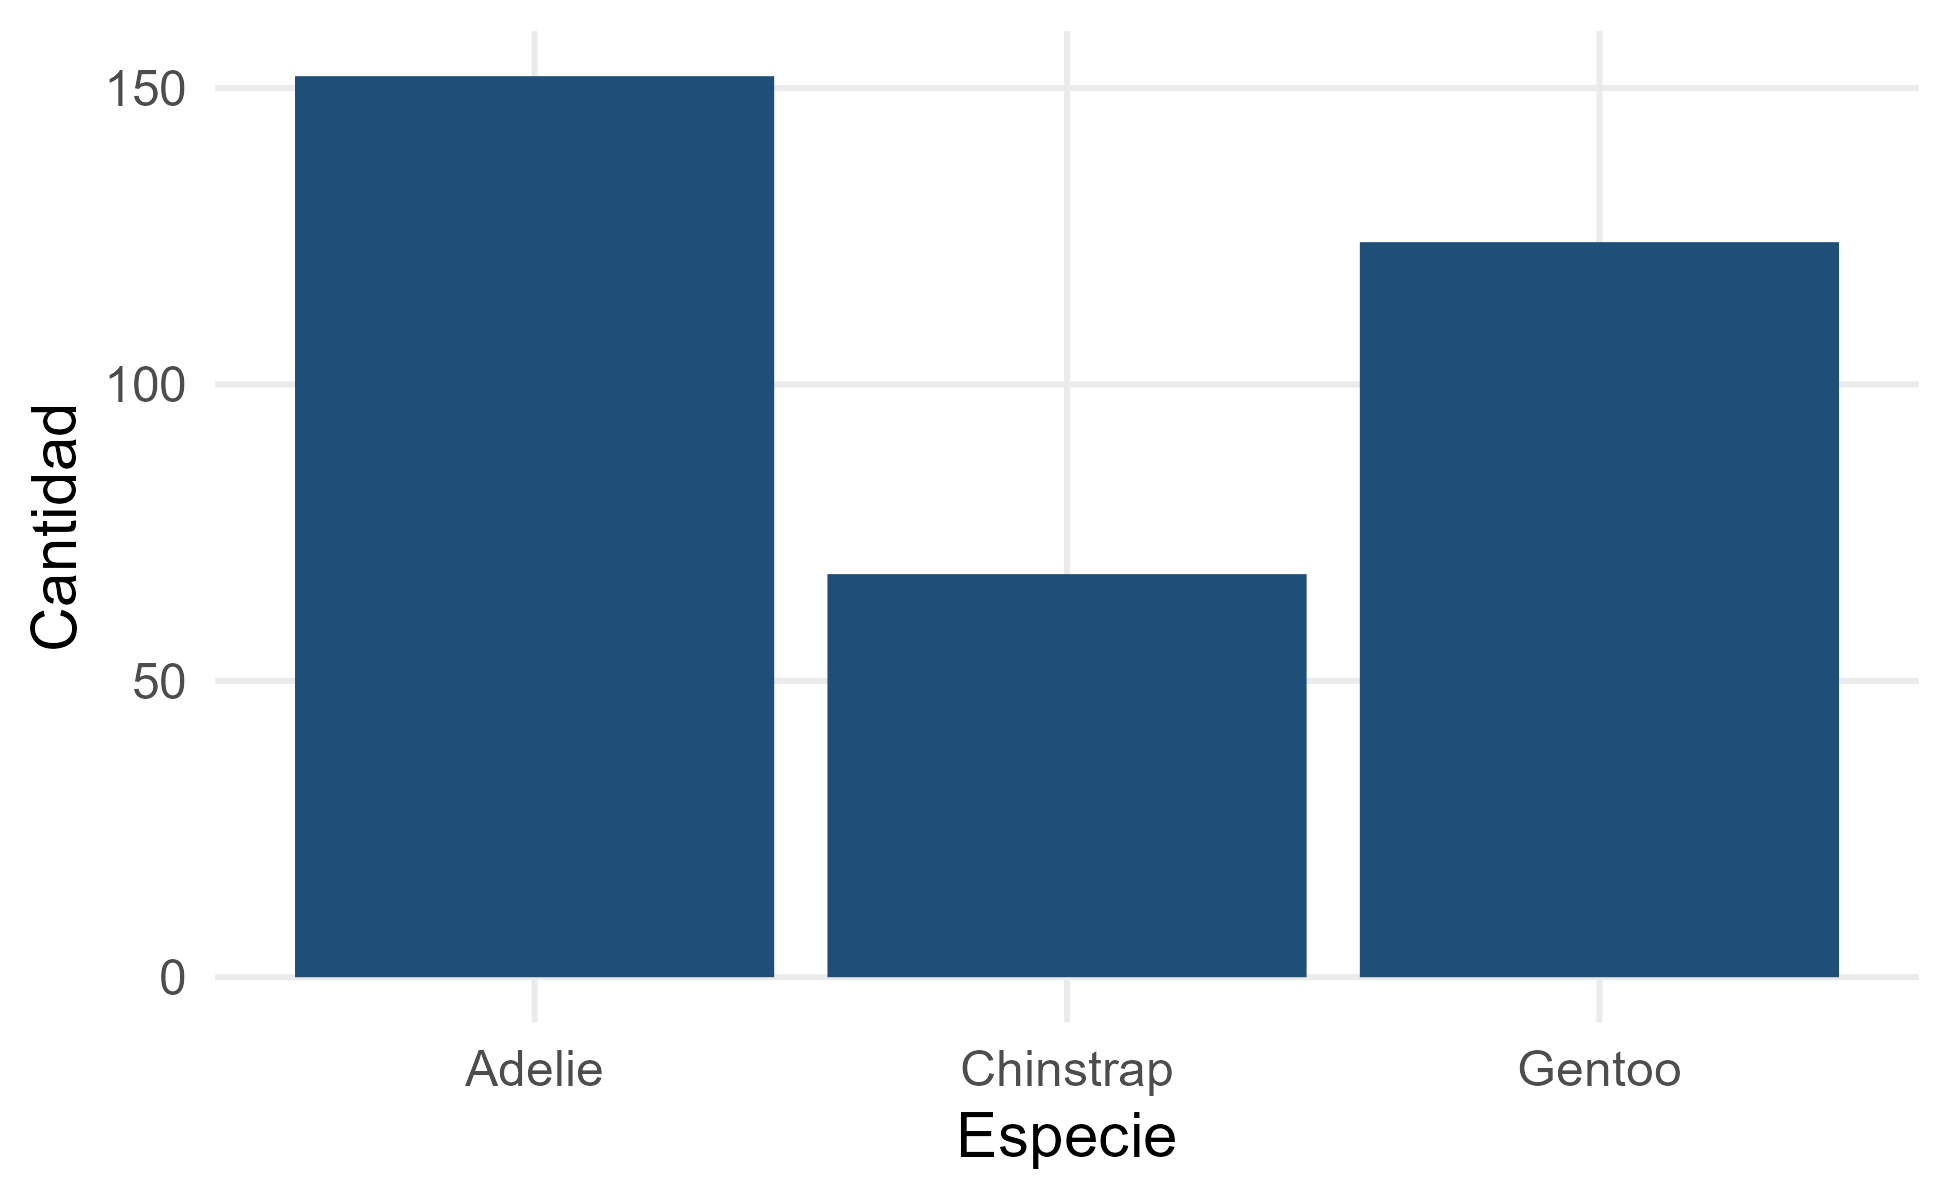
\includegraphics[width=0.95\textwidth]{r-barras-especie.png}%
      }{%
        \begin{tikzpicture}[scale=0.72]
          \draw[grisT,->] (0,0) -- (0,3.3);
          \draw[grisT,->] (0,0) -- (4.6,0);
          \fill[azulUS] (0.5,0) rectangle (1.3,3.0);
          \fill[azulUS] (1.7,0) rectangle (2.5,1.5);
          \fill[azulUS] (2.9,0) rectangle (3.7,2.2);
          \node[below,font=\tiny] at (0.9,0) {Adelia};
          \node[below,font=\tiny] at (2.1,0) {Barbijo};
          \node[below,font=\tiny] at (3.3,0) {Juanito};
          \node[left,font=\tiny] at (0,3.0) {152};
          \node[left,font=\tiny] at (0,1.5) {68};
        \end{tikzpicture}%
      }\\[3pt]
      {\scriptsize Diagrama de barras}
    \end{column}
    \begin{column}{0.48\textwidth}
      \textbf{Variable cuantitativa}\\[4pt]
      La pregunta es \emph{¿cómo se distribuyen los valores?}\\[6pt]
      \centering
      \IfFileExists{figuras/r-histograma-masa.png}{%
        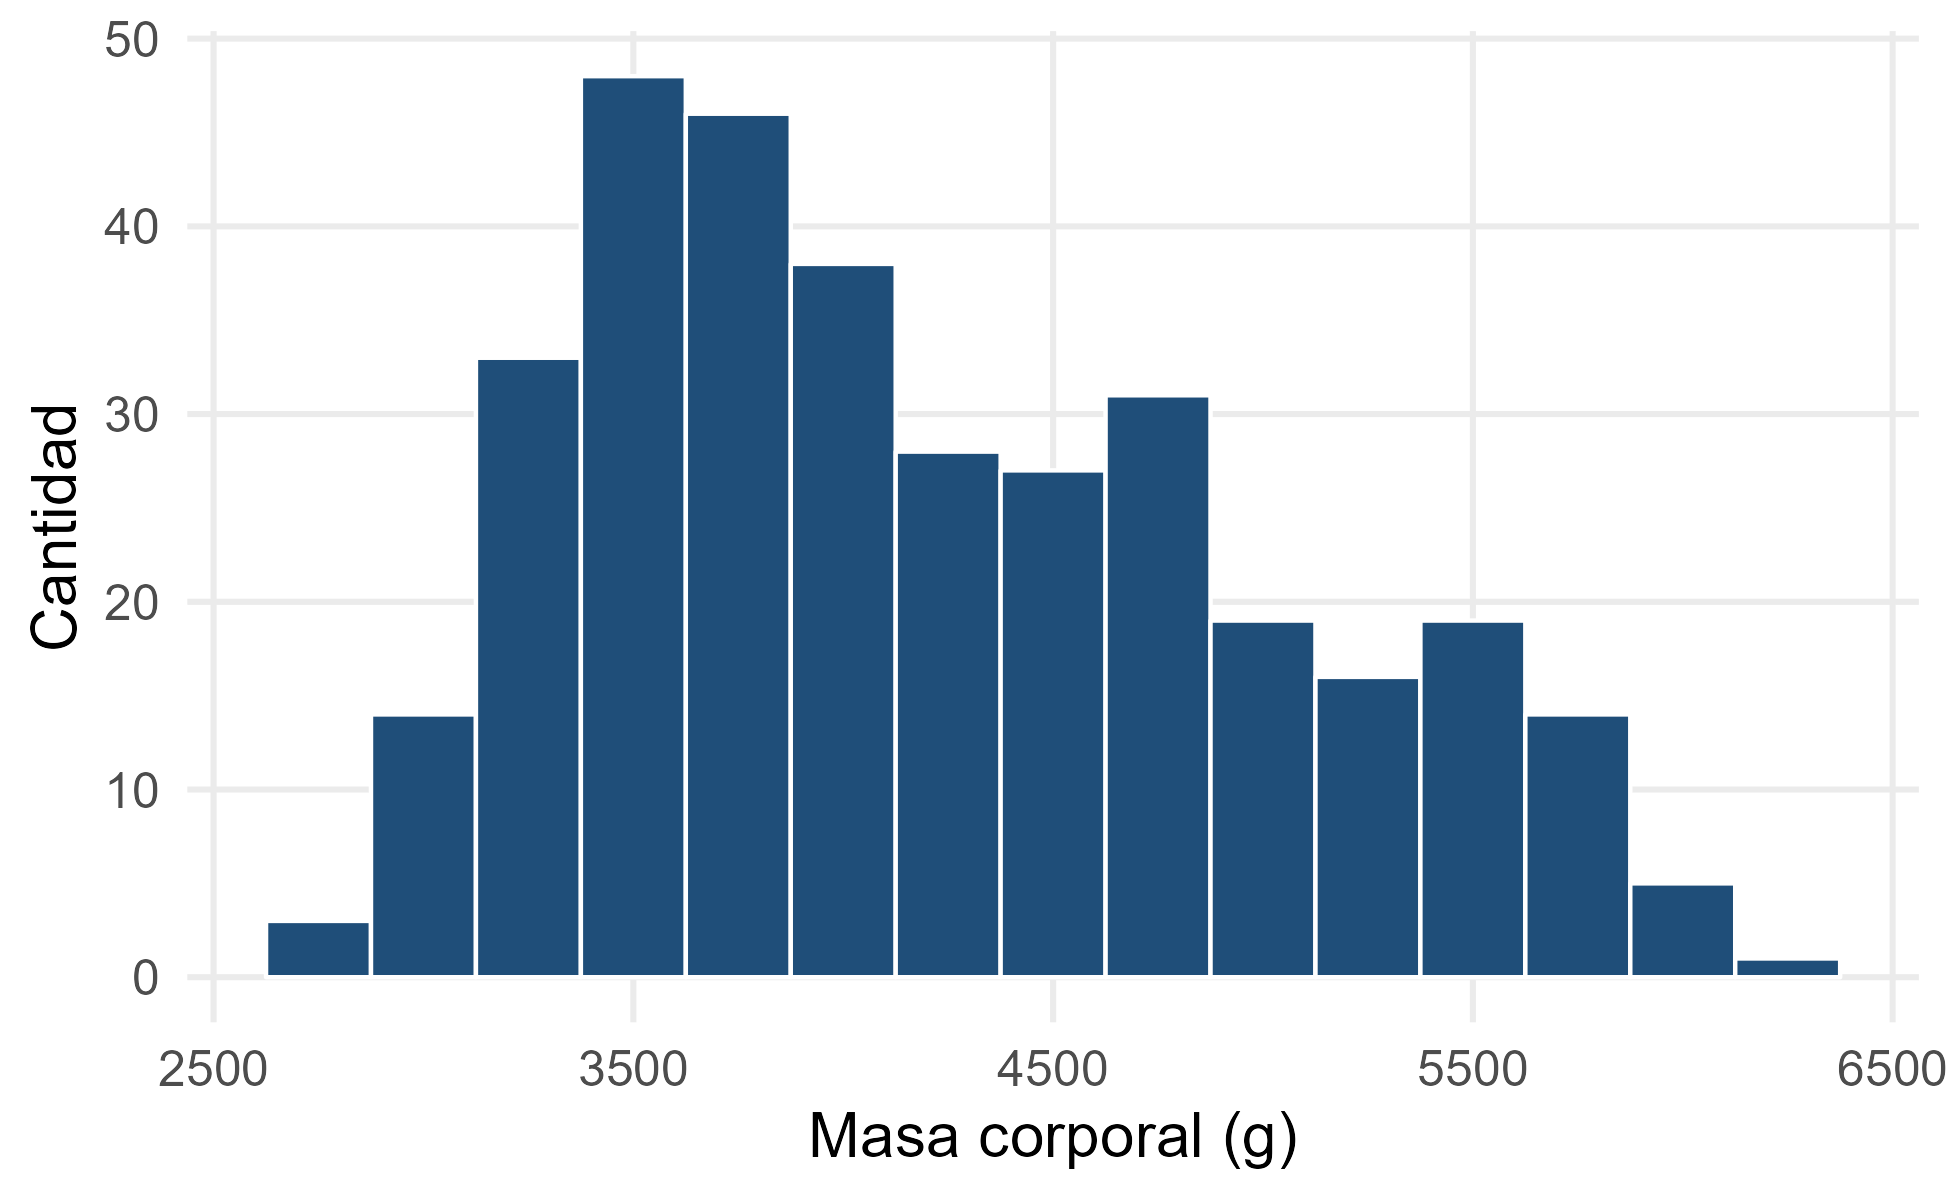
\includegraphics[width=0.95\textwidth]{r-histograma-masa.png}%
      }{%
        \begin{tikzpicture}[scale=0.72]
          \draw[grisT,->] (0,0) -- (0,3.3);
          \draw[grisT,->] (0,0) -- (4.6,0);
          \fill[azulUS] (0.3,0) rectangle (0.75,0.8);
          \fill[azulUS] (0.75,0) rectangle (1.2,2.1);
          \fill[azulUS] (1.2,0) rectangle (1.65,2.7);
          \fill[azulUS] (1.65,0) rectangle (2.1,1.6);
          \fill[azulUS] (2.1,0) rectangle (2.55,0.9);
          \fill[azulUS] (2.55,0) rectangle (3.0,1.7);
          \fill[azulUS] (3.0,0) rectangle (3.45,2.3);
          \fill[azulUS] (3.45,0) rectangle (3.9,1.1);
          \fill[azulUS] (3.9,0) rectangle (4.35,0.4);
          \node[below,font=\tiny] at (2.3,0) {masa corporal (g)};
        \end{tikzpicture}%
      }\\[3pt]
      {\scriptsize Histograma}
    \end{column}
  \end{columns}

  \vspace{0.4cm}
  \destaca{\small ¿Notan algo raro en el histograma? Tiene \textbf{dos montículos}.
  Eso casi siempre significa que hay grupos distintos mezclados.}
\end{frame}
% ============================================================
\begin{frame}[fragile]{Esas gráficas, en R}
  Las tres gráficas de esta unidad salen con la misma estructura. Se dice qué tabla se
  usa, qué variable va en cada eje y qué figura se dibuja.

\begin{lstlisting}
library(ggplot2)

ggplot(penguins, aes(x = species)) +          # una categorica
  geom_bar()

ggplot(penguins, aes(x = body_mass_g)) +      # una cuantitativa
  geom_histogram(binwidth = 250)

ggplot(penguins, aes(x = body_mass_g, fill = species)) +
  geom_histogram(binwidth = 250)              # separando por especie
\end{lstlisting}

  \vspace{0.2cm}
  \destaca{\small El signo \Rc{+} encadena capas, y hace en \texttt{ggplot2} el mismo
  papel que \Rc{|>} en \texttt{dplyr}. Primero se declara con \Rc{aes()} qué variable va
  a dónde, y después se agrega la figura con un \Rc{geom\_}.

  \vspace{0.15cm}
  Nótese que \Rc{binwidth} es el ancho de clase. Es un valor que elegimos nosotros, no
  algo que R descubra en los datos.}
\end{frame}
\begin{frame}{Al leer un histograma, tres preguntas}
  \begin{columns}[T]
    \begin{column}{0.3\textwidth}
      \destaca{\centering\textbf{Centro}\\[3pt]{\small ¿Alrededor de qué valor se acumulan?}}
    \end{column}
    \begin{column}{0.3\textwidth}
      \destaca{\centering\textbf{Dispersión}\\[3pt]{\small ¿Qué tan esparcidos están?}}
    \end{column}
    \begin{column}{0.3\textwidth}
      \destaca{\centering\textbf{Forma}\\[3pt]{\small ¿Simétrica? ¿Sesgada? ¿Uno o varios picos?}}
    \end{column}
  \end{columns}

  \vspace{0.8cm}
  \destaca{Y una cuarta pregunta, que se trata en la diapositiva siguiente. ¿Cuánto
  del dibujo depende del \textbf{ancho de clase} que elegimos?}
\end{frame}
\begin{frame}{De dónde venían los dos montículos}
  \centering
  \IfFileExists{figuras/r-histograma-especie.png}{%
    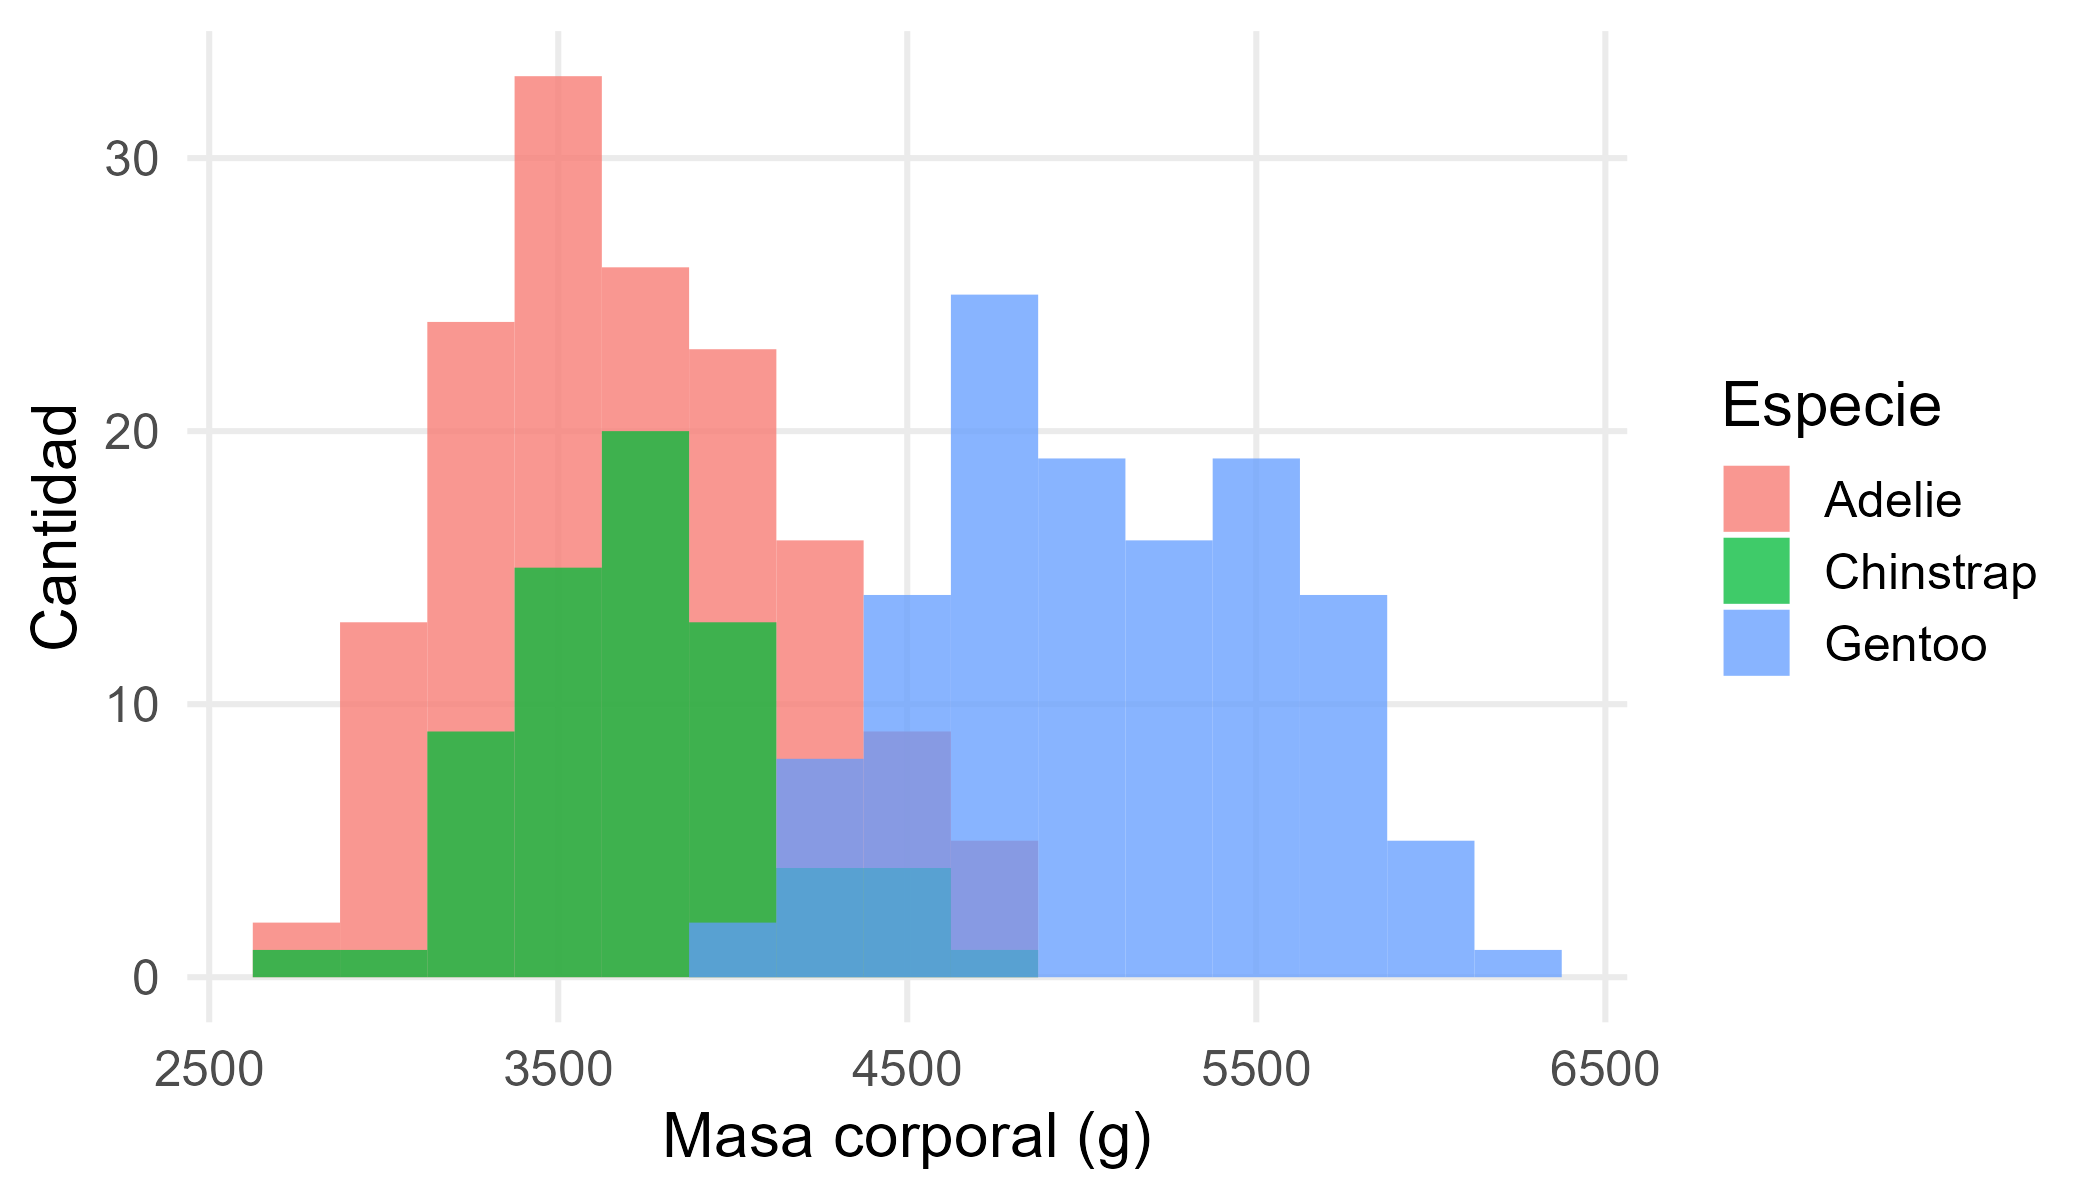
\includegraphics[width=0.78\textwidth]{r-histograma-especie.png}
  }{%
    {\color{grisT}\small[Histograma de la masa separado por especie]}
  }

  \vspace{0.3cm}
  \raggedright
  \destaca{Al separar por especie, el misterio se resuelve. Los Juanito son
  notablemente más pesados. Los ``dos montículos'' eran \textbf{dos poblaciones
  mezcladas}.

  \vspace{0.2cm}
  Moraleja para todo el curso: cuando una distribución se ve rara, casi siempre hay
  una \textbf{variable escondida} que la explica. Buscarla es parte del análisis.}
\end{frame}
\begin{frame}{El ancho de clase no es un detalle}
  \centering
  \IfFileExists{figuras/r-ancho-100.png}{%
    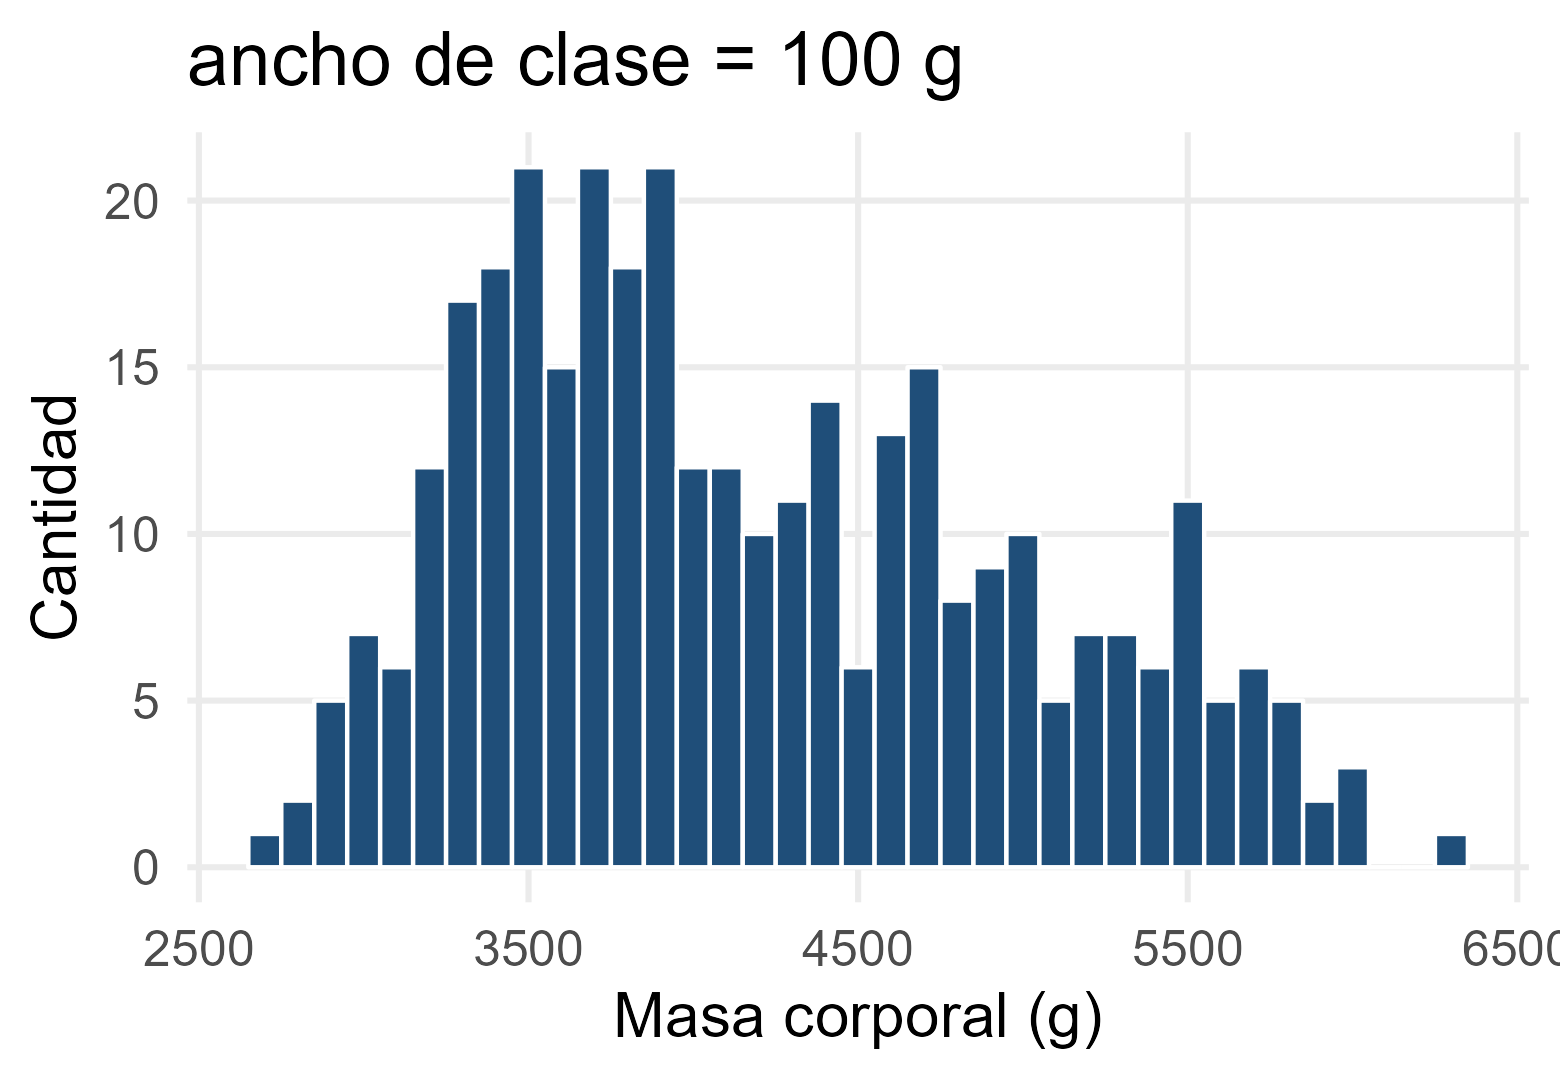
\includegraphics[width=0.32\textwidth]{r-ancho-100.png}\hfill
    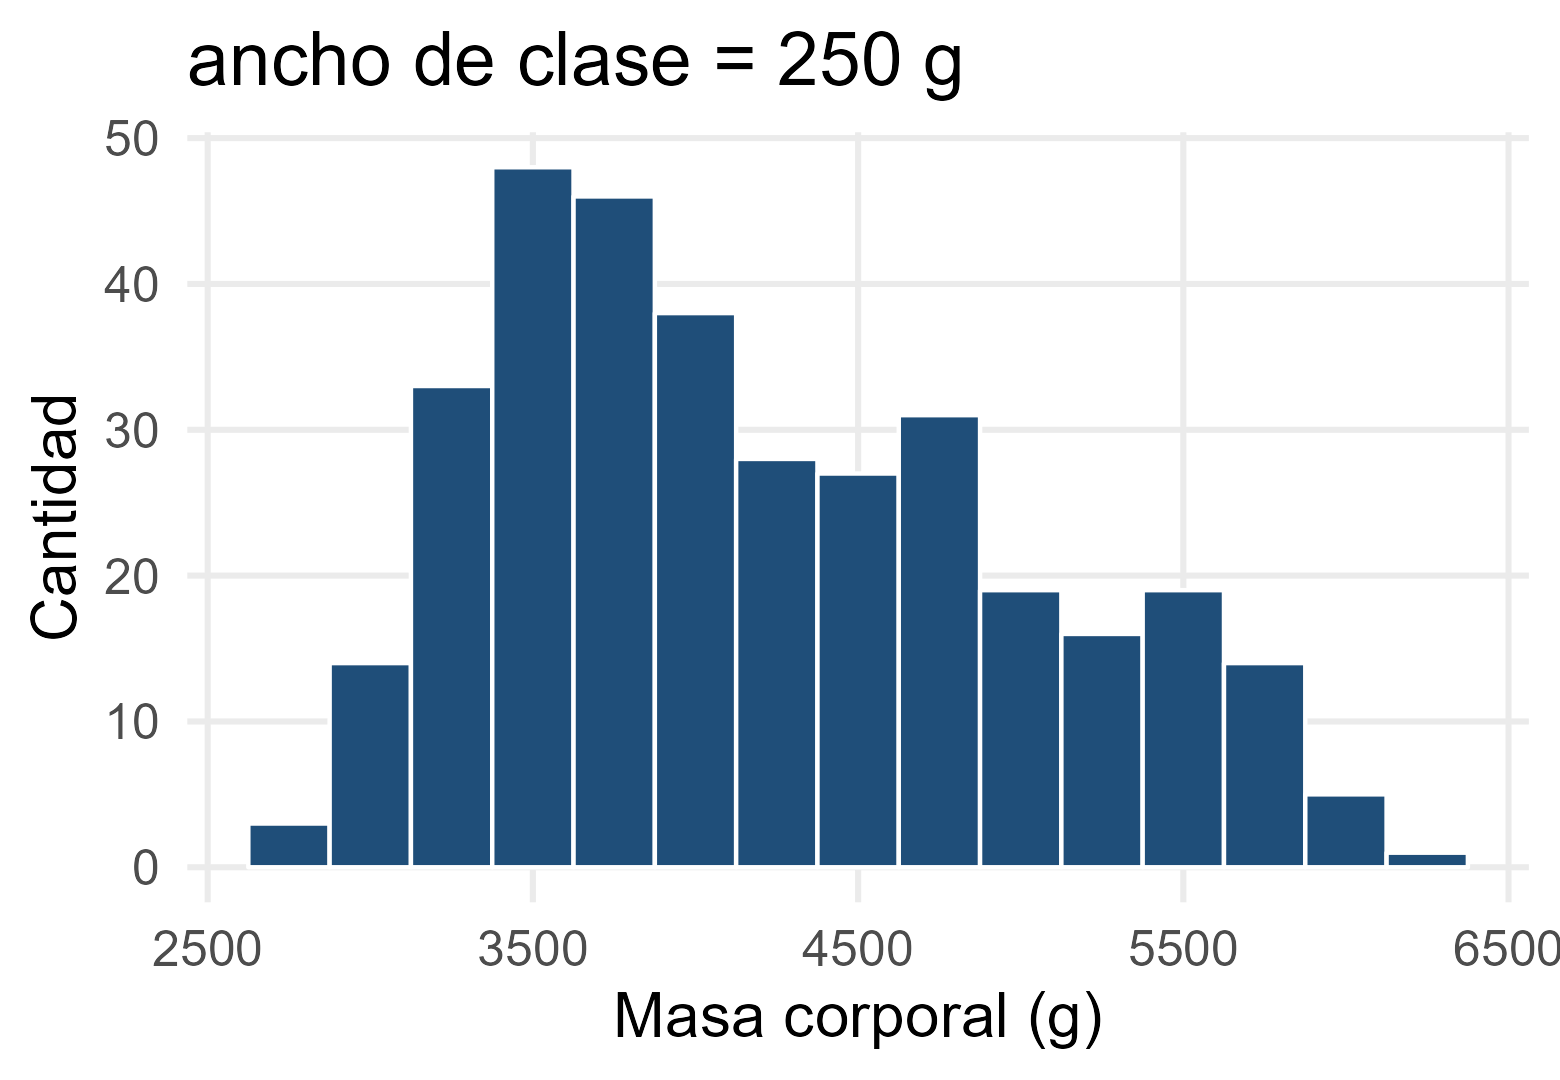
\includegraphics[width=0.32\textwidth]{r-ancho-250.png}\hfill
    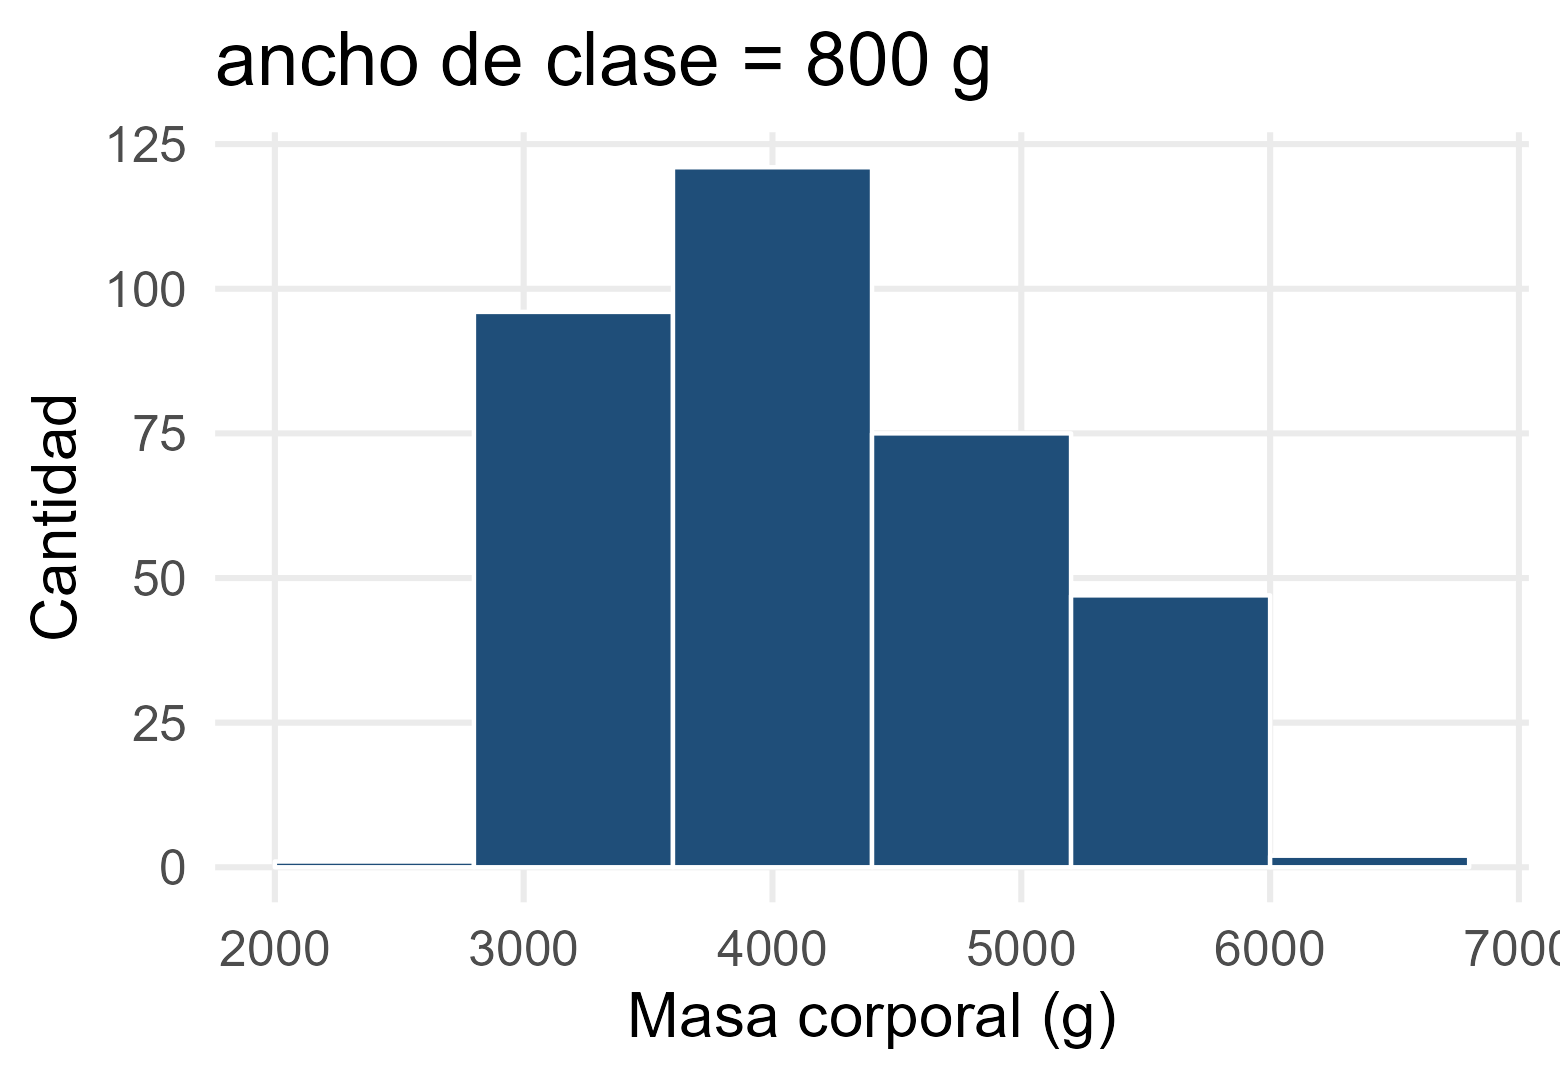
\includegraphics[width=0.32\textwidth]{r-ancho-800.png}
  }{%
    {\color{grisT}\small[Tres histogramas de los mismos datos con anchos de clase distintos]}
  }

  \vspace{0.35cm}
  \raggedright
  \destaca{Los \textbf{mismos datos}, tres decisiones distintas. Con intervalos muy
  angostos solo se ve ruido; con intervalos muy anchos desaparece la estructura; en
  medio se distinguen los dos grupos.

  \vspace{0.2cm}
  Un histograma no es un dato objetivo: es una \textbf{decisión} de quien grafica.
  En el libro hay un laboratorio para moverlo y verlo en vivo.}
\end{frame}
% ============================================================
% ============================================================
\begin{frame}[fragile]{Práctica de la unidad}
  {\small\color{grisT} En clase, con la computadora abierta. No se entrega.}

  \vspace{0.2cm}
  Sobre \texttt{penguins}, en un script nuevo.

  \vspace{0.25cm}
  \begin{enumerate}
    \item Clasificar las ocho columnas por tipo y por escala, anotando la tabla como comentario
    \item Una gráfica de barras de \Rc{island} y un histograma de \Rc{flipper\_length\_mm}
    \item Repetir el histograma con tres anchos de clase distintos. ¿Cuál cuenta mejor la historia?
    \item Separar ese histograma por especie con \Rc{fill}. ¿Aparecen grupos?
    \item Escribir en dos renglones si el estudio de Palmer fue observacional o experimental, y por qué
  \end{enumerate}

  \vspace{0.3cm}
  \destaca{\small El punto 3 no tiene una respuesta única, y ese es el punto. Se pide
  justificar la elección, no acertarla.

  \vspace{0.15cm}
  El punto 5 se contesta con una sola pregunta. ¿Quién asignó la especie y el sexo de
  cada pingüino?}
\end{frame}
\begin{frame}{Cierre de la unidad}
  \textbf{Lo que vimos}
  \begin{itemize}
    \item Individuos y variables. Siempre hay que identificarlos antes de calcular
    \item Tipos de variables y escalas de medición
    \item Observacional contra experimental, y por qué solo el segundo permite hablar de causa
    \item La gráfica que corresponde a cada tipo de variable, y cómo se hace en R
  \end{itemize}

  \vspace{0.4cm}
  \textbf{Pendientes de la semana}
  \begin{itemize}
    \item El cuestionario de la unidad en Moodle, que ya está abierto
    \item La práctica de la semana, que se entrega el viernes
  \end{itemize}

  \vspace{0.5cm}
  \destaca{\small Son dos pendientes, y no más. El capítulo 1 del libro está ahí para
  consultarlo cuando algo no quede claro, con sus ejercicios y sus soluciones
  explicadas, pero no es tarea con fecha.}
\end{frame}
% ============================================================
\section{Unidad 2: Estadística descriptiva}
% ---------- bloque: medidas de localización ----------
\begin{frame}[plain]
  \hojaSesion{Unidad 2: describir con números}{%
  Ya sabemos mirar una distribución. Ahora la resumimos en unos pocos números.
  Media, mediana y moda. Cuál de ellas resiste un valor extremo y cuál no, y cómo se
  calculan a mano y en R.}
\end{frame}
% ============================================================
\begin{frame}{Del dibujo al número}
  El histograma de la unidad anterior contestaba tres preguntas. Dónde está el centro,
  qué tan dispersos están los datos y qué forma tienen.

  \vspace{0.35cm}
  \destaca{Una gráfica se ve, pero no se puede escribir en un renglón de una tabla ni
  meter en una prueba estadística. Para eso hacen falta \textbf{números que resuman} la
  distribución.}

  \vspace{0.35cm}
  Esta unidad convierte cada una de esas tres preguntas en un número. Empezamos por el
  centro, que es la que se contesta con las medidas de \textbf{localización}.
\end{frame}
% ============================================================
\begin{frame}{Tres maneras de decir dónde está el centro}
  \begin{columns}[T]
    \begin{column}{0.32\textwidth}
      \destaca{\centering\textbf{Media}\\[4pt]
      {\small El promedio. Reparte el total entre todos por igual.}\\[6pt]
      $\bar{x} = \dfrac{1}{n}\displaystyle\sum_{i=1}^{n} x_i$}
    \end{column}
    \begin{column}{0.32\textwidth}
      \destaca{\centering\textbf{Mediana}\\[4pt]
      {\small El valor de en medio, con los datos ordenados. Deja la mitad de cada
      lado.}}
    \end{column}
    \begin{column}{0.32\textwidth}
      \destaca{\centering\textbf{Moda}\\[4pt]
      {\small El valor que más se repite. Puede haber más de una, o ninguna útil.}}
    \end{column}
  \end{columns}

  \vspace{0.5cm}
  \destaca{Las tres contestan la misma pregunta y casi nunca dan el mismo número.
  Elegir cuál reportar es una decisión, y como toda decisión del curso, conviene poder
  justificarla.}
\end{frame}
% ============================================================
\begin{frame}[fragile]{Las tres, en R}
\begin{lstlisting}
mean(penguins$body_mass_g, na.rm = TRUE)      # media
median(penguins$body_mass_g, na.rm = TRUE)    # mediana

table(penguins$species)                       # la moda de una categorica
names(which.max(table(penguins$species)))     # la categoria mas frecuente
\end{lstlisting}

  \vspace{0.25cm}
  \destaca{\small R no trae una función para la moda, y la ausencia dice algo. En una
  variable cuantitativa continua casi ningún valor se repite, así que la moda no informa
  gran cosa. Donde sí sirve es en las \textbf{categóricas}, y ahí se lee directo de
  \Rc{table()}.

  \vspace{0.15cm}
  Nótese que \Rc{na.rm = TRUE} vuelve a aparecer. Con faltantes en la columna, sin él,
  las dos primeras líneas devuelven \Rc{NA}.}
\end{frame}
% ============================================================
\begin{frame}[fragile]{Cuál resiste un valor extremo}
  Supongamos que al capturar la masa de cinco pingüinos se cuela un error de dedo.

\begin{lstlisting}
masa <- c(3750, 3800, 3250, 3450, 4500)
mean(masa)     # 3750
median(masa)   # 3750

masa[5] <- 45000     # se tecleo un cero de mas
mean(masa)     # 11850
median(masa)   # 3750
\end{lstlisting}

  \vspace{0.25cm}
  \destaca{\small Un solo dato mal capturado multiplicó la media por más de tres, y a la
  mediana no la movió ni un gramo. Se dice que la mediana es \textbf{robusta} y la media
  no lo es.

  \vspace{0.15cm}
  De ahí una costumbre que conviene adoptar. Cuando la media y la mediana se separan
  mucho, algo pasa en los datos, y vale la pena ir a ver qué. A veces es un error de
  captura y a veces es una distribución sesgada de verdad.}
\end{frame}
% ============================================================
\begin{frame}{Cuál reportar}
  \begin{center}
  {\small
  \begin{tabular}{@{}p{5.2cm}p{3.2cm}p{4.4cm}@{}}
    \toprule
    \textbf{Si la distribución} & \textbf{Conviene} & \textbf{Por qué} \\
    \midrule
    Es aproximadamente simétrica y sin valores extremos & Media &
      Usa toda la información y es la que entra en casi toda la inferencia \\
    Está sesgada o tiene valores extremos & Mediana &
      No se deja arrastrar por unos pocos datos \\
    Es categórica & Moda &
      Es la única de las tres que tiene sentido \\
    \bottomrule
  \end{tabular}}
  \end{center}

  \vspace{0.4cm}
  \destaca{Este es el primer renglón que aportamos al \textbf{mapa de decisión} con una
  medida numérica. La pregunta era ``¿cuál es el centro de esta variable?'' y la
  respuesta depende del tipo de variable y de la forma de la distribución, no del gusto
  de quien reporta.}
\end{frame}
% ============================================================
\begin{frame}{El mismo cálculo a mano}
  Con cinco valores ya ordenados, $3250$, $3450$, $3750$, $3800$ y $4500$ gramos.

  \vspace{0.3cm}
  \begin{columns}[T]
    \begin{column}{0.48\textwidth}
      \textbf{Media}\\[4pt]
      $\bar{x} = \dfrac{3250+3450+3750+3800+4500}{5} = \dfrac{18750}{5} = 3750$
      \vspace{0.3cm}

      \textbf{Mediana con $n$ impar}\\[4pt]
      El valor de la posición $\frac{n+1}{2} = 3$, es decir $3750$.
    \end{column}
    \begin{column}{0.48\textwidth}
      \textbf{Mediana con $n$ par}\\[4pt]
      Si se quita el $4500$ quedan cuatro valores. Se promedian los dos centrales.
      \[ \frac{3450+3750}{2} = 3600 \]
      Y la media pasa a ser $14250/4 = 3562.5$.
    \end{column}
  \end{columns}

  \vspace{0.4cm}
  \destaca{\small Vale la pena hacerlo una vez a mano y comprobarlo con R. En el examen
  se pide sobre conjuntos pequeños como este, con el formulario a la vista.}
\end{frame}
% ============================================================
\begin{frame}[fragile]{Resúmenes por grupo}
  Un promedio general casi nunca es la respuesta interesante. Lo que suele importar es
  cómo cambia de un grupo a otro.

\begin{lstlisting}
penguins |>
  group_by(species) |>
  summarise(n      = n(),
            media  = mean(body_mass_g, na.rm = TRUE),
            mediana = median(body_mass_g, na.rm = TRUE))
\end{lstlisting}

  \vspace{0.25cm}
  \destaca{\small Es la misma tubería de la semana pasada, con dos resúmenes en lugar de
  uno. La función \Rc{n()} cuenta cuántos hay en cada grupo, y conviene incluirla
  siempre. Un promedio calculado sobre tres individuos no merece la misma confianza que
  uno calculado sobre ciento veinticuatro.

  \vspace{0.15cm}
  Al ver la tabla completa se entiende de dónde venían los dos montículos del histograma
  de la unidad anterior.}
\end{frame}
% ============================================================
\begin{frame}[fragile]{Práctica de la semana}
  {\small\color{grisT} Se entrega en Teams antes de la próxima clase. Es la única entrega de la semana.}

  \vspace{0.2cm}
  Sobre \texttt{penguins}, en el script de la unidad.

  \vspace{0.25cm}
  \begin{enumerate}
    \item Media y mediana del largo de la aleta. ¿Se parecen? ¿Qué sugiere eso sobre la forma?
    \item Las dos, ahora por especie, con \Rc{group\_by()} y \Rc{summarise()}, incluyendo \Rc{n()}
    \item Cambiar a mano un valor de la masa por uno absurdo y recalcular media y mediana
    \item ¿Cuál es la isla más frecuente? ¿Qué medida de centro se está usando al contestar?
  \end{enumerate}

  \vspace{0.3cm}
  \destaca{\small El punto 3 se hace sobre una copia de la columna, no sobre
  \texttt{penguins}. Los datos originales no se tocan nunca, y esa es una regla de
  higiene que vale para todo el curso.}
\end{frame}
\begin{frame}[plain]
  \centering

  \vspace{1.0cm}
  \IfFileExists{figuras/lter_penguins.png}{%
    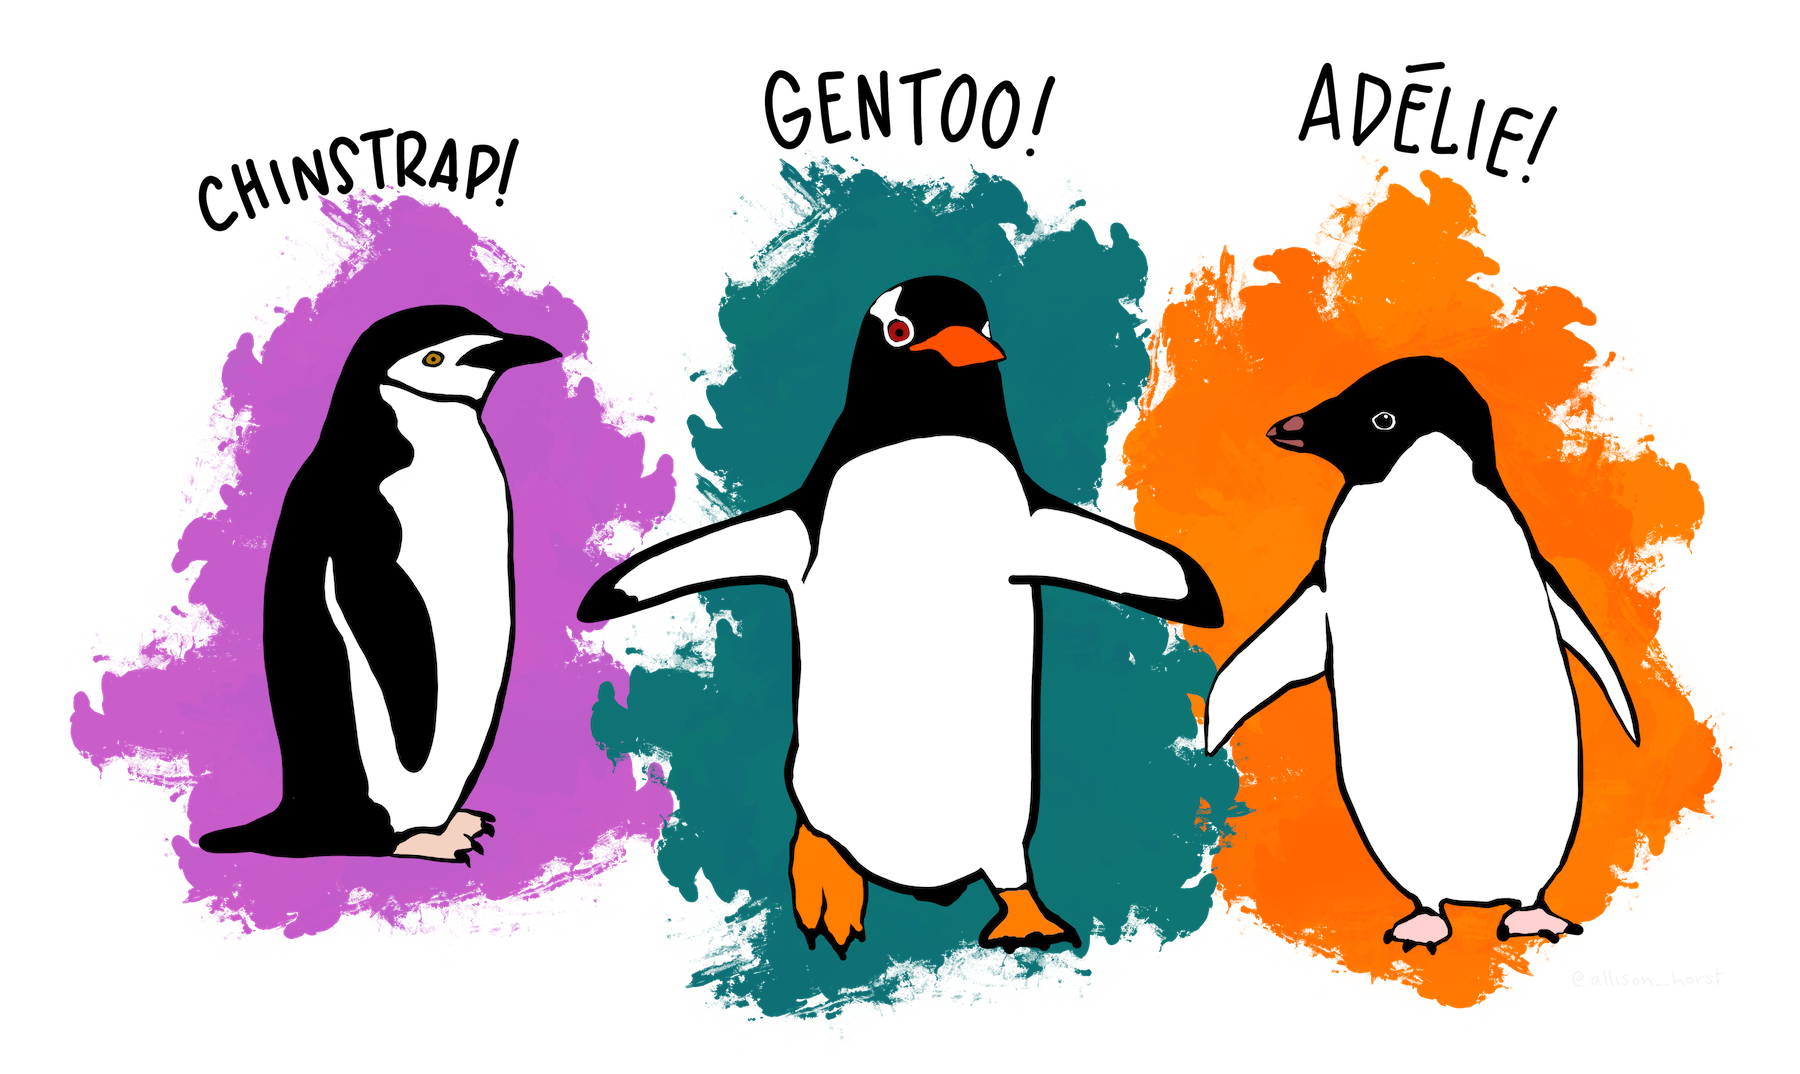
\includegraphics[height=0.36\textheight]{lter_penguins.png}\\[2pt]
    \creditoHorst
  }{%
    \begin{tikzpicture}[scale=0.8]
      \begin{scope}[shift={(-2.4,0)}] \pingAdelie \end{scope}
      \begin{scope}[shift={(0,0)}] \pingChinstrap \end{scope}
      \begin{scope}[shift={(2.4,0)}] \pingGentoo \end{scope}
    \end{tikzpicture}
  }

  \vspace{0.6cm}
  {\Large\color{azulUS} ¿Preguntas?}\\[10pt]
  {\small\color{grisT} \url{https://rosaliahdez.github.io/notas-estadistica/} \\
  Comunicación por Teams · Cuestionarios en Moodle}

  \vspace{0.7cm}
  {\tiny\color{grisT}
  Datos: Horst A, Hill A, Gorman K (2020). \textit{palmerpenguins} (CC-0). ---
  Estudio original: Gorman KB, Williams TD, Fraser WR (2014).
  \textit{Ecological sexual dimorphism and environmental variability within a community
  of Antarctic penguins (genus Pygoscelis)}. PLoS ONE 9(3):e90081. ---
  Ilustraciones: \textit{Artwork by @allison\_horst}.}
\end{frame}
\end{document}
